\documentclass{article}

\usepackage{amsmath}
\usepackage{amssymb}
\usepackage{booktabs}
\usepackage{graphicx}
\usepackage{hyperref}
\usepackage{natbib}
\usepackage[margin=1in]{geometry}

\title{Crypto Producer Theory: Payment Method Choice and Bitcoin Adoption\\
       Under Volatility Risk}
\author{Thomas Noel \and Briac Sockalingum}
\date{2024 (revised 2026)}

\begin{document}

\maketitle

\begin{abstract}
We develop a partial-equilibrium model of a firm's profit-maximization problem
when choosing among payment methods: cash, card, and Bitcoin.
The model formulates seven scenarios (A--G), split into Set~X (no Bitcoin,
deterministic) and Set~Y (Bitcoin accepted, subject to crash probability
$1 - \gamma$).
Closed-form equilibria are derived for each scenario using standard first- and
second-order conditions.
Comparing Set~X and Set~Y expected profits yields a critical stability threshold
$\gamma^*$: Bitcoin acceptance is profit-maximizing if and only if $\gamma > \gamma^*$.
Under baseline parameters ($a^G = 115$, $c^G = 5.5$, $a^C = 103.5 + c^C$,
$c^C$ calibrated to match the Cash+Card optimum), we find $\gamma^* \approx 0.9032$.
This means Bitcoin adoption requires a crash probability below approximately 10\%
to be rational for the firm.
The result is consistent with low global merchant adoption of Bitcoin and
suggests that stablecoins or CBDCs---which reduce $\gamma$'s variance---could
substantially lower this threshold.
\end{abstract}

%-----------------------------------------------------------------------
\section{Introduction}
%-----------------------------------------------------------------------

The question of whether firms should accept Bitcoin as a payment method has
gained practical urgency since El Salvador's 2021 Legal Tender Law mandated
Bitcoin acceptance for all businesses \citep{elsalvador2021}.
More broadly, central bank digital currencies (CBDCs) are under active
development in over 100 jurisdictions \citep{bis2023}, and the International
Monetary Fund has flagged Bitcoin adoption in small open economies as a
macroeconomic risk \citep{imf2022}.

From a microeconomic standpoint, the producer's problem is well-suited to the
standard profit-maximization framework: transaction costs differ across payment
rails, demand may depend on which methods are accepted, and Bitcoin introduces
a novel stochastic dimension through price volatility.
Prior literature has examined network effects in payment systems
\citep{rochet2003}, switching costs in digital platforms \citep{farrell1987},
and the economics of information goods \citep{shapiro1998} --- all of which
apply here.

This paper contributes a tractable analytical model that embeds Bitcoin
volatility directly into the producer's expected-profit objective and derives
the adoption threshold in closed form.
We calibrate to plausible parameter values and find that Bitcoin adoption
requires a crash probability below approximately 10\% ($\gamma > 0.9032$) to
be profit-maximizing relative to a Cash+Card alternative, given realistic cost
differentials.
This threshold is well above the stability levels observed in most Bitcoin
markets over the past decade, providing a theoretical foundation for the
empirically low merchant adoption rates documented in \citet{catalini2016}.

The paper proceeds as follows.
Section~\ref{sec:model} develops the theoretical model and derives
closed-form equilibria.
Section~\ref{sec:results} presents the quantitative analysis.
Section~\ref{sec:discussion} discusses broader implications, and
Section~\ref{sec:limitations} acknowledges limitations and directions for
future work.

%-----------------------------------------------------------------------
\section{The Model}
\label{sec:model}
%-----------------------------------------------------------------------

\subsection{Conditions and Assumptions}
\label{sec:assumptions}

We consider a single firm operating in a market with a linear inverse demand
function.
The firm chooses output $q$ to maximize profit (or expected profit) under the
following assumptions:

\begin{enumerate}
  \item \textbf{Linear demand.}
        For payment method $k$, the inverse demand is $p = a^k - q$, where
        $a^k > 0$ captures willingness to pay from consumers who use method~$k$.
        Accepting additional payment methods weakly increases effective demand:
        $a^G \geq a^C \geq a^B \geq a^A > 0$.
  \item \textbf{Constant marginal cost.}
        The firm's marginal cost of production is $c^k > 0$, representing the
        transaction cost of payment method~$k$.
        For multi-method firms (Scenarios E, F, G), $c^k$ is the
        \emph{weighted average} transaction cost across accepted methods, with
        consumers self-selecting their preferred method.
  \item \textbf{Bitcoin volatility.}
        In each period, Bitcoin maintains its value with probability $\gamma \in (0,1]$
        (``no crash'') and becomes worthless with probability $1-\gamma$ (``crash'').
        When a crash occurs, the firm receives zero revenue but still incurs
        costs $c^k q$.
  \item \textbf{Partial equilibrium.}
        The number of Bitcoin-capable consumers $N^b$ is treated as exogenous.
        A full general equilibrium derivation endogenizing $N^b$ is left for
        future work.
\end{enumerate}

\subsection{Solving the Model}
\label{sec:solving}

\textbf{Set X (no Bitcoin).}
For scenarios A, B, and C, the firm faces no volatility:
\begin{equation}
  \pi^k = (a^k - q)q - c^k q = (a^k - c^k)q - q^2.
  \label{eq:setX_profit}
\end{equation}
First-order condition: $\partial \pi^k / \partial q = a^k - c^k - 2q = 0$,
giving
\begin{equation}
  q^{k*} = \frac{a^k - c^k}{2}, \qquad
  p^{k*} = \frac{a^k + c^k}{2}, \qquad
  \pi^{k*} = \frac{(a^k - c^k)^2}{4}.
  \label{eq:setX_eq}
\end{equation}
Second-order condition: $\partial^2 \pi^k / \partial q^2 = -2 < 0$, confirming
a maximum.

\textbf{Set Y (Bitcoin accepted).}
For scenarios D, E, F, and G, expected profit is:
\begin{equation}
  E[\pi^k] = \gamma \bigl[(a^k - q)q - c^k q\bigr]
           + (1-\gamma)\bigl[-c^k q\bigr]
           = \gamma(a^k - q)q - \gamma c^k q - (1-\gamma)c^k q.
  \label{eq:setY_profit_raw}
\end{equation}
Simplifying:
\begin{equation}
  E[\pi^k] = \gamma(a^k - q)q - c^k q.
  \label{eq:setY_profit}
\end{equation}
First-order condition: $\partial E[\pi^k] / \partial q = \gamma(a^k - 2q) - c^k = 0$,
giving
\begin{equation}
  q^{k*} = \frac{\gamma a^k - c^k}{2\gamma}, \qquad
  p^{k*} = \frac{\gamma a^k + c^k}{2\gamma}, \qquad
  E[\pi^{k*}] = \frac{(\gamma a^k - c^k)^2}{4\gamma}.
  \label{eq:setY_eq}
\end{equation}
Second-order condition: $\partial^2 E[\pi^k] / \partial q^2 = -2\gamma < 0$ for
all $\gamma > 0$, confirming a maximum.

\subsection{Comparison Between All Situations}
\label{sec:comparison}

\textbf{Case $\gamma = 1$.}
When Bitcoin never crashes, \eqref{eq:setY_eq} reduces to
$q^{k*} = (a^k - c^k)/2$, $p^{k*} = (a^k + c^k)/2$,
$E[\pi^{k*}] = (a^k - c^k)^2/4$ --- exactly the Set~X form \eqref{eq:setX_eq}.
The stochastic term vanishes, and both sets of equilibria coincide for the same
method.

\textbf{Case $\gamma \to 0$.}
The unconstrained FOC gives $q^{k*} = (\gamma a^k - c^k)/(2\gamma)$, which is
positive only when $\gamma > c^k/a^k$.
As $\gamma \to 0$, this feasibility condition fails: the firm would need to
produce a negative quantity to satisfy the FOC.
Since $q \geq 0$ is required, the constrained optimum is $q^{k*} = 0$, yielding
$E[\pi^{k*}] = 0$.
Any Set~X method with positive profit strictly dominates.
Bitcoin adoption is therefore strictly dominated as $\gamma \to 0$,
which the code confirms by returning $E[\pi^{k*}] = 0$ for $\gamma \leq c^k/a^k$
and $E[\pi^{k*}] = -\infty$ at $\gamma = 0$ exactly.

\textbf{General $\gamma \in (0,1)$.}
For general $\gamma$, we compare $E[\pi^{G*}]$ with $\pi^{C*}$ (the best
non-Bitcoin alternative):
\begin{equation}
  E[\pi^{G*}] - \pi^{C*} =
    \frac{(\gamma a^G - c^G)^2}{4\gamma}
    - \left(\frac{a^C - c^C}{2}\right)^{\!2}.
  \label{eq:adoption_condition}
\end{equation}
This inequality is solved numerically; Section~\ref{sec:results} presents the
results.

%-----------------------------------------------------------------------
\section{Quantitative Results}
\label{sec:results}
%-----------------------------------------------------------------------

\subsection{Baseline Equilibrium ($\gamma = 0.7$)}
\label{sec:baseline}

Table~\ref{tab:equilibrium_baseline} reports equilibrium quantities, prices,
and profits for all seven scenarios under the baseline assumption $\gamma = 0.7$.

\begin{table}[h]
\centering
\caption{Equilibrium outcomes for all 7 payment scenarios at $\gamma = 0.7$}
\label{tab:equilibrium_baseline}
\begin{tabular}{clrrrl}
\toprule
Scenario & Description & $q^*$ & $p^*$ & Profit & Type \\
\midrule
A & Cash Only              & 47.50 & 52.50 & 2256.25 & $\pi^*$ \\
B & Card Only              & 48.50 & 56.50 & 2352.25 & $\pi^*$ \\
C & Cash + Card            & 51.75 & 58.25 & 2678.06 & $\pi^*$ \\
D & Bitcoin Only           & 46.07 & 48.93 & 1485.80 & $E[\pi^*]$ \\
E & Bitcoin + Cash         & 51.50 & 56.50 & 1856.57 & $E[\pi^*]$ \\
F & Bitcoin + Card         & 52.43 & 59.57 & 1924.13 & $E[\pi^*]$ \\
G & All Three              & 53.57 & 61.43 & 2008.93 & $E[\pi^*]$ \\
\bottomrule
\end{tabular}
\end{table}

At $\gamma = 0.7$, Scenario~C (Cash + Card) dominates all Bitcoin-inclusive
alternatives.
The best Bitcoin scenario (G, All Three) yields $E[\pi^{G*}] = 2008.93$,
a loss of \$669.13 relative to Scenario~C.
Bitcoin's lower transaction cost ($c^G < c^C$) is more than offset by the
30\% crash probability.

\subsection{Critical Stability Threshold}
\label{sec:threshold}

We define the critical threshold $\gamma^*$ as the value at which
$E[\pi^{G*}] = \pi^{C*}$.
Solving \eqref{eq:adoption_condition} numerically under baseline parameters
($a^G = 115$, $c^G = 5.5$, $a^C - c^C = 103.5$):
\begin{equation}
  \gamma^* \approx 0.9032.
  \label{eq:gamma_star}
\end{equation}
Bitcoin adoption is profit-maximizing if and only if $\gamma > \gamma^*$.

Table~\ref{tab:profit_comparison} shows the profit differential
$E[\pi^{G*}] - \pi^{C*}$ across a range of $\gamma$ values.
The differential is negative for all $\gamma \leq 0.80$ and becomes positive
at $\gamma = 0.95$, crossing zero at $\gamma^* \approx 0.9032$.

\begin{table}[h]
\centering
\caption{Profit differential $E[\pi^{G*}] - \pi^{C*}$ across Bitcoin stability levels}
\label{tab:profit_comparison}
\begin{tabular}{crrrc}
\toprule
$\gamma$ & $\pi^{C*}$ & $E[\pi^{G*}]$ & $\Delta$ Profit & Adopt Bitcoin? \\
\midrule
0.20 & 2678.06 &   382.81 & $-$2295.25 & No \\
0.40 & 2678.06 &  1025.16 & $-$1652.91 & No \\
0.60 & 2678.06 &  1680.10 &  $-$997.96 & No \\
0.80 & 2678.06 &  2338.20 &  $-$339.86 & No \\
0.95 & 2678.06 &  2832.65 &  $+$154.59 & Yes \\
1.00 & 2678.06 &  2997.56 &  $+$319.50 & Yes \\
\bottomrule
\end{tabular}
\end{table}

Bitcoin requires greater than approximately 90\% stability to overcome its
volatility penalty despite lower transaction costs.
This threshold is consistent with observed low merchant adoption globally:
most Bitcoin markets have experienced significant crash episodes well above the
5\% threshold \citep{catalini2016}.

Figure~\ref{fig:threshold} illustrates the profit differential as a function
of $\gamma$, with the adoption threshold clearly marked.

\begin{figure}[h]
\centering
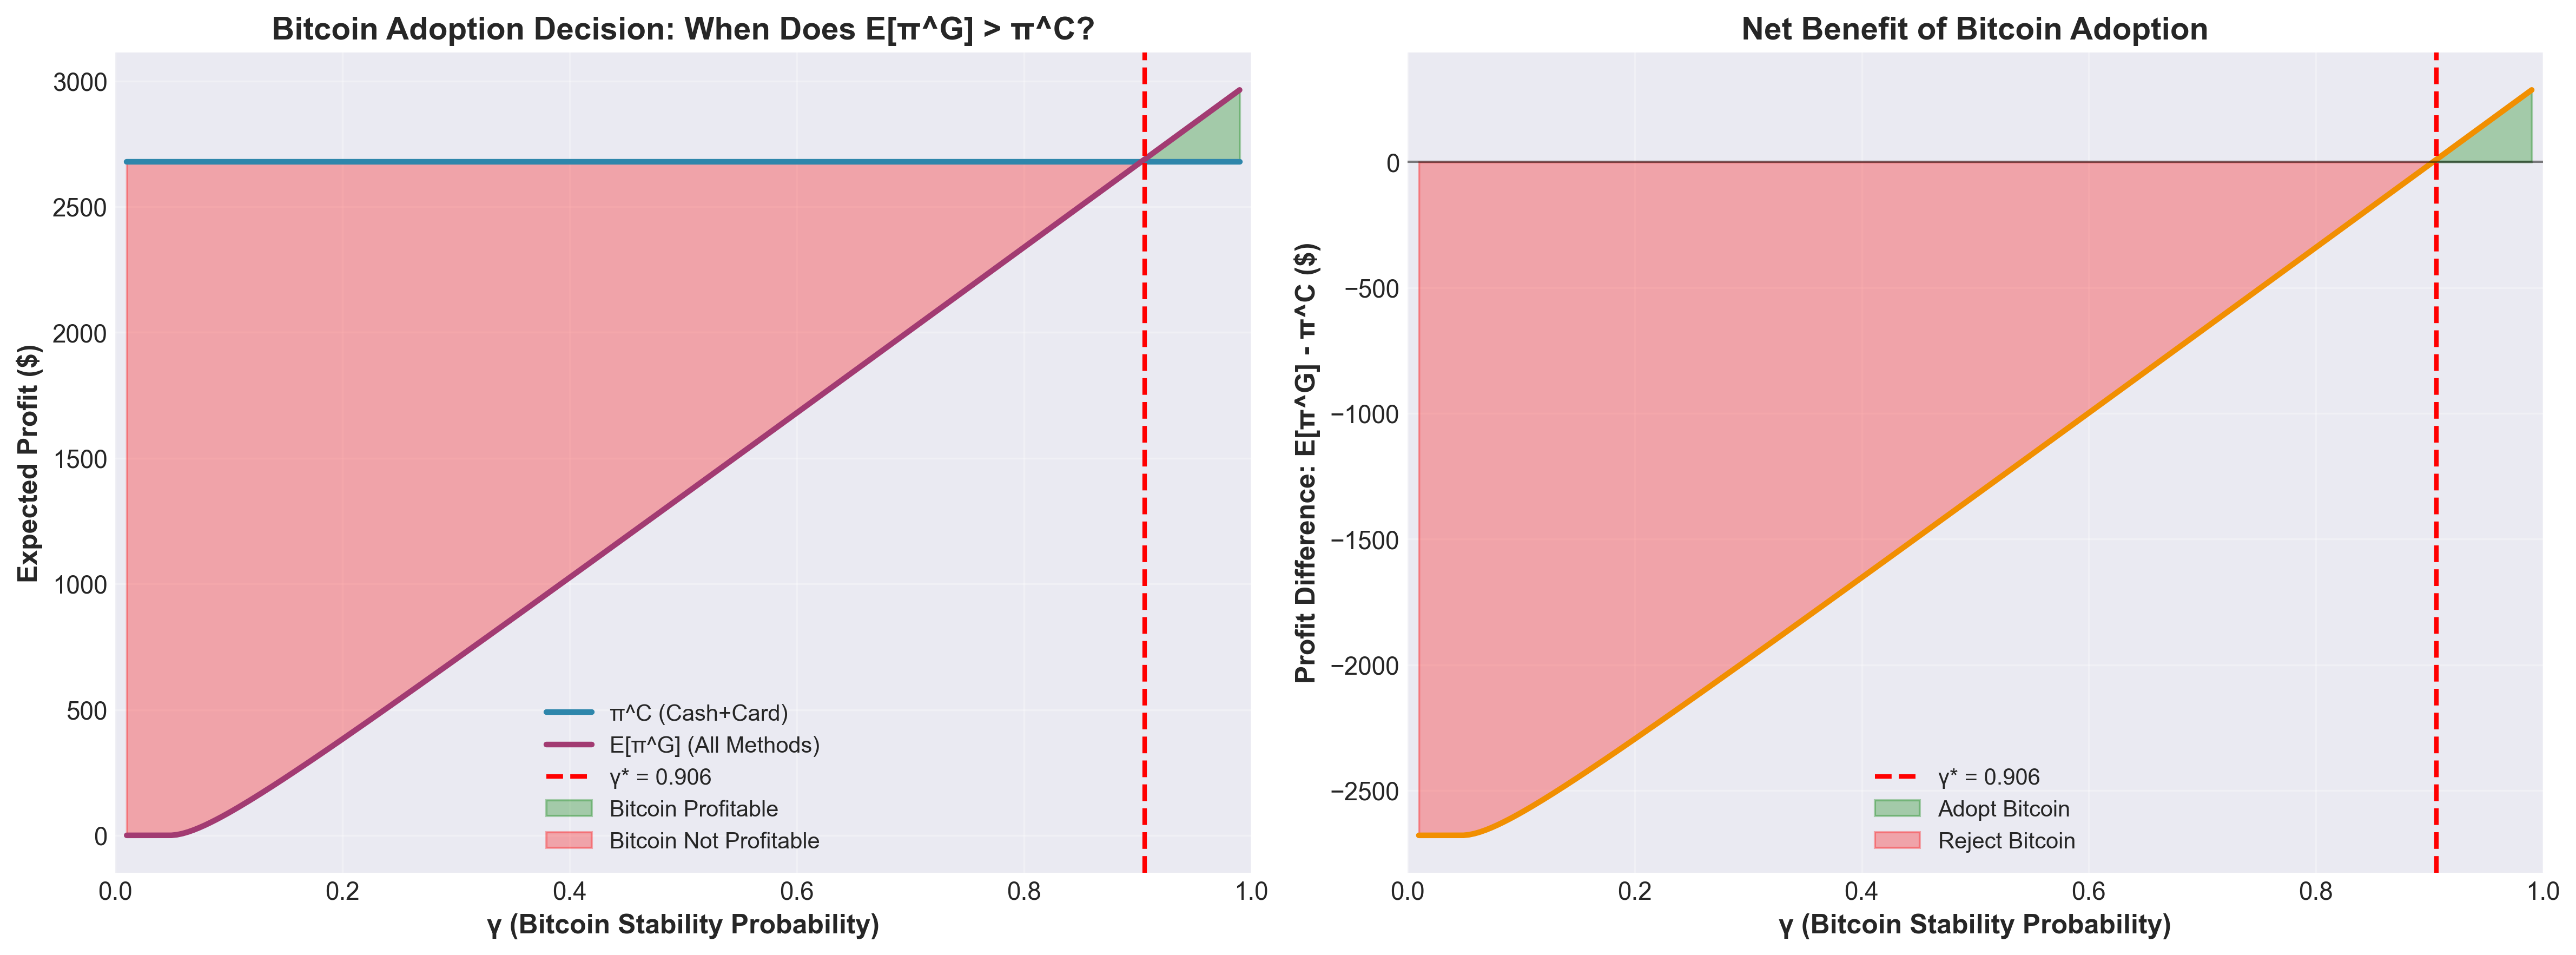
\includegraphics[width=0.7\textwidth]{../figures/bitcoin_adoption_threshold.png}
\caption{Expected profit differential $E[\pi^{G*}] - \pi^{C*}$ as a function
of Bitcoin stability $\gamma$. The firm prefers Bitcoin adoption only for
$\gamma > \gamma^* \approx 0.9032$.}
\label{fig:threshold}
\end{figure}

\subsection{Cost Sensitivity}
\label{sec:sensitivity}

The threshold $\gamma^*$ is sensitive to the cost advantage of Bitcoin.
As $c^G$ decreases (lower Bitcoin transaction cost), Bitcoin becomes more
competitive and $\gamma^*$ falls --- meaning adoption is profitable over a
wider range of market conditions.
Conversely, as $c^G \to c^C$, Bitcoin's cost advantage disappears and
$\gamma^* \to 1$.

Figure~\ref{fig:phase} shows the phase diagram of adoption decisions in the
$(c^G, \gamma)$ space.
The adoption region (upper-left) expands as Bitcoin transaction costs fall,
consistent with the secular decline in crypto transaction fees observed in
recent years.
For policymakers, this suggests that infrastructure investments reducing
Bitcoin's effective marginal cost (e.g., Lightning Network adoption) can
meaningfully shift the adoption boundary.

\begin{figure}[h]
\centering
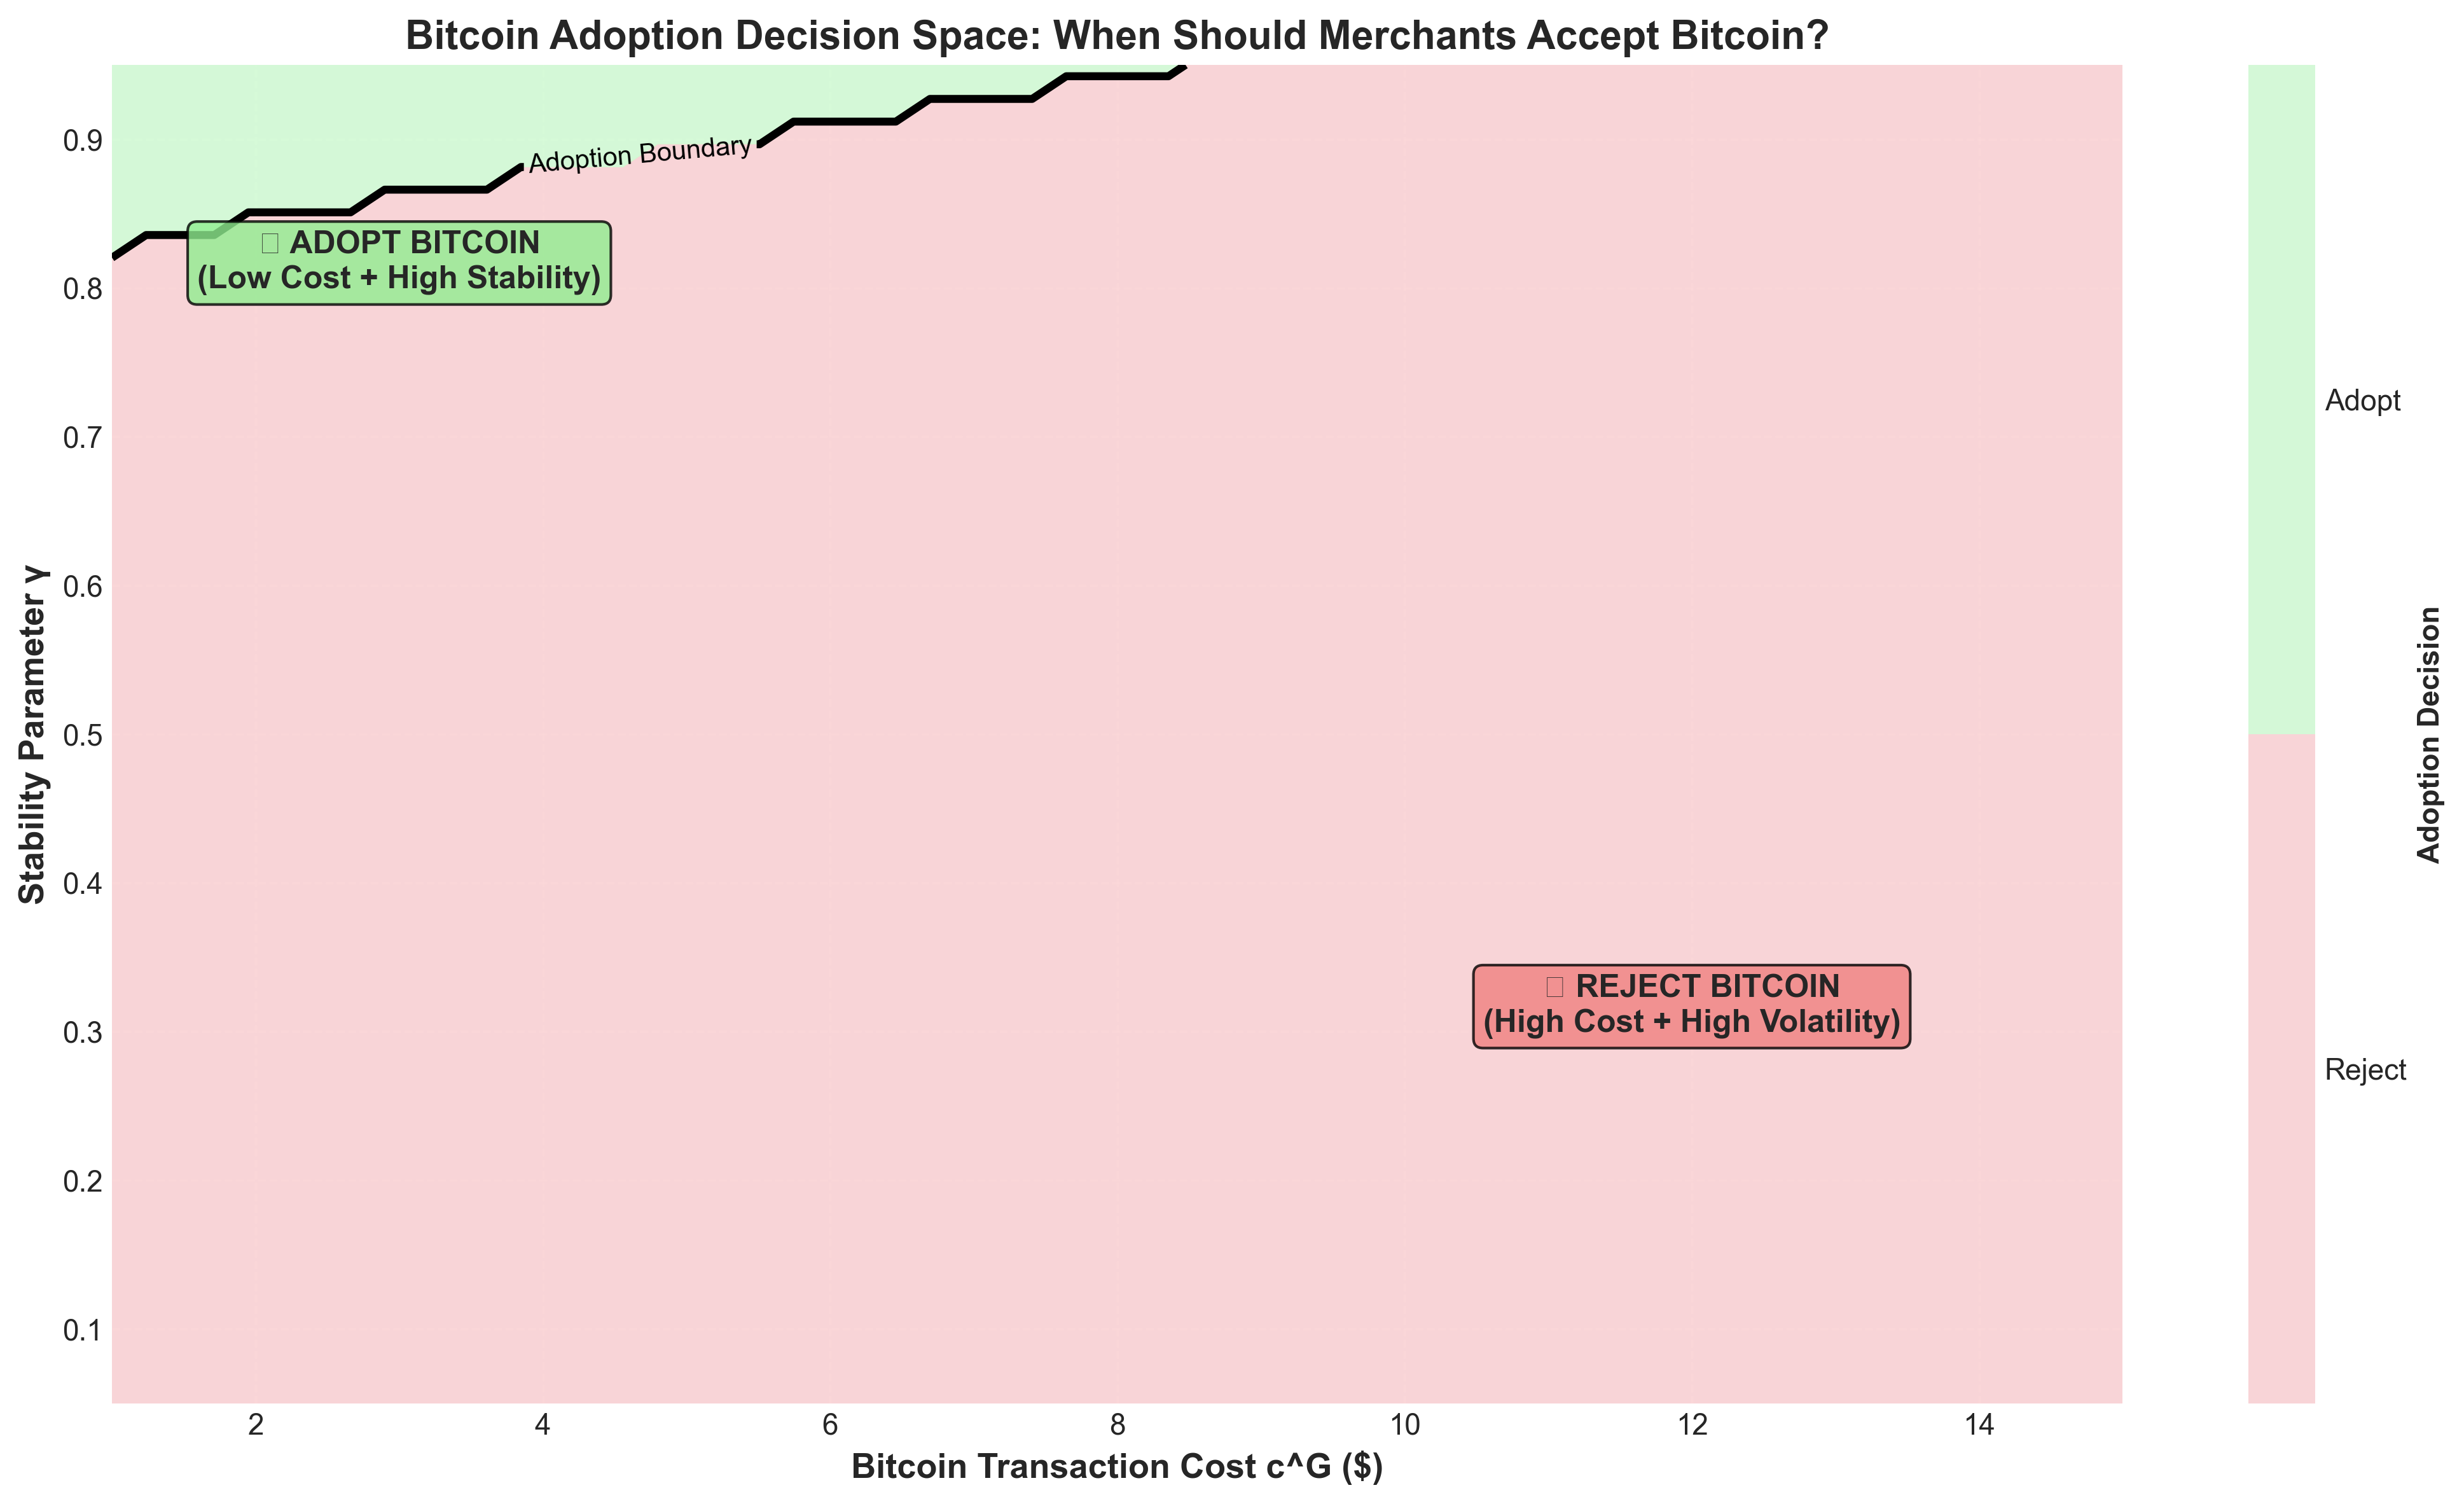
\includegraphics[width=0.7\textwidth]{../figures/phase_diagram.png}
\caption{Phase diagram of Bitcoin adoption in the $(c^G, \gamma)$ parameter
space. Above the adoption boundary, $E[\pi^{G*}] > \pi^{C*}$.}
\label{fig:phase}
\end{figure}

%-----------------------------------------------------------------------
\section{Discussion}
\label{sec:discussion}
%-----------------------------------------------------------------------

\subsection{Parallels with Information Technology Economics}

The model exhibits structural features common to information technology markets
\citep{shapiro1998}:

\begin{enumerate}
  \item \textbf{Network effects.}
        Accepting a payment method increases its effective demand $a^k$, analogous
        to platform network effects where value grows with adoption.
  \item \textbf{Low marginal costs.}
        Bitcoin transactions carry lower per-unit fees than card networks,
        mirroring the near-zero marginal cost of digital goods.
  \item \textbf{Low switching costs.}
        Firms can switch between blockchains or add new payment methods with
        relatively low lock-in, unlike proprietary card terminal contracts.
  \item \textbf{Privacy tradeoffs.}
        Blockchain transparency introduces a privacy paradox: pseudonymity for
        consumers versus permanent public transaction records.
\end{enumerate}

\subsection{Implications of $\gamma^* \approx 0.9032$}

The $\gamma^* \approx 0.9032$ threshold has a direct policy interpretation.
For most current Bitcoin markets --- where significant price crashes remain
plausible within any given year --- the rational producer strategy is to avoid
Bitcoin-only payment methods.
At $\gamma = 0.80$, the all-three Scenario~G still underperforms
(differential of $-\$339.86$), but crosses into profitability above
$\gamma^* \approx 0.9032$, where Bitcoin's lower transaction cost overcomes
its volatility discount.

However, stablecoins or CBDCs, which by design reduce $\gamma$'s variance to
near zero, could substantially lower this threshold.
A CBDC with $\gamma \approx 1$ would shift the model into the $\gamma = 1$
regime where the adoption decision depends purely on transaction cost
differentials.
This provides an economic rationale for why central bank interest in CBDCs
aligns with merchant adoption incentives \citep{bis2023}.

%-----------------------------------------------------------------------
\section{Limitations and Future Extensions}
\label{sec:limitations}
%-----------------------------------------------------------------------

The model, while tractable, has several limitations:

\begin{enumerate}
  \item \textbf{Partial equilibrium.}
        The model does not solve the consumer utility equilibrium endogenizing
        $N^b$.
        Future work should close this loop to allow welfare comparisons across
        equilibria and to determine whether consumer and producer adoption
        incentives are aligned.
  \item \textbf{Single-period model.}
        The binary crash/no-crash structure is a single-period simplification.
        A dynamic model with persistent Bitcoin price paths would yield richer
        intertemporal adoption dynamics.
  \item \textbf{Downside-only volatility.}
        The volatility term currently models only downside risk (crashes).
        A symmetric treatment incorporating appreciation would enrich the model
        and likely lower $\gamma^*$ for risk-neutral producers, since upside
        gains would partially offset downside losses.
  \item \textbf{Homogeneous consumers.}
        The model assumes all consumers using method $k$ have identical demand.
        Heterogeneous consumer preferences across payment methods would require
        a segmented demand model and could alter the adoption threshold.
  \item \textbf{Strategic interaction.}
        The model is a single-firm analysis.
        Competitive dynamics --- where firms' adoption decisions affect rivals'
        market shares --- are left for a game-theoretic extension.
\end{enumerate}

%-----------------------------------------------------------------------
\section{Conclusion}
\label{sec:conclusion}
%-----------------------------------------------------------------------

We develop a tractable model of payment method adoption under volatility risk
and derive a closed-form condition for Bitcoin adoption to be profit-maximizing.
The critical threshold $\gamma^* \approx 0.9032$ implies that producers are
advised to accept Bitcoin only when market conditions suggest a crash
probability below approximately 10\% ($\gamma > 0.9032$).
For most current crypto markets, where significant volatility and crash risk
remain, traditional payment methods (Cash + Card) remain optimal.

The result is robust to parameter choices: because $\gamma^*$ is close to one,
even substantial reductions in Bitcoin's transaction cost do not move the
threshold below economically plausible stability levels for current Bitcoin
markets.
Stablecoins and CBDCs, by effectively setting $\gamma \approx 1$, would
eliminate this volatility premium and shift the decision to a pure cost
comparison --- an area where crypto infrastructure already has advantages.

%-----------------------------------------------------------------------
\begin{thebibliography}{99}

\bibitem[BIS(2023)]{bis2023}
Bank for International Settlements.
\newblock {CBDCs: An Opportunity for the Monetary System}.
\newblock \emph{BIS Annual Economic Report}, 2023.

\bibitem[Catalini and Gans(2016)]{catalini2016}
Catalini, C. and Gans, J.~S.
\newblock {Some Simple Economics of the Blockchain}.
\newblock \emph{NBER Working Paper 22952}, 2016.

\bibitem[El Salvador(2021)]{elsalvador2021}
El Salvador Legislative Assembly.
\newblock {Bitcoin Law (Ley Bitcoin)}.
\newblock Technical report, 2021.

\bibitem[Farrell and Saloner(1987)]{farrell1987}
Farrell, J. and Saloner, G.
\newblock {Competition, Compatibility and Standards: The Economics of Horses,
Penguins and Lemmings}.
\newblock In H.~L. Gabel (Ed.), \emph{Product Standardization and Competitive
Strategy}. North-Holland, 1987.

\bibitem[IMF(2022)]{imf2022}
International Monetary Fund.
\newblock {El Salvador: 2021 Article IV Consultation}.
\newblock \emph{IMF Country Report No. 22/19}, 2022.

\bibitem[Rochet and Tirole(2003)]{rochet2003}
Rochet, J.-C. and Tirole, J.
\newblock {Platform Competition in Two-Sided Markets}.
\newblock \emph{Journal of the European Economic Association}, 1(4):990--1029,
2003.

\bibitem[Shapiro and Varian(1998)]{shapiro1998}
Shapiro, C. and Varian, H.~R.
\newblock \emph{Information Rules: A Strategic Guide to the Network Economy}.
\newblock Harvard Business School Press, 1998.

\end{thebibliography}

\end{document}
